\documentclass{article}
\usepackage{tikz}
\begin{document}
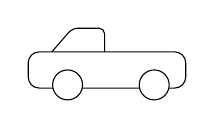
\begin{tikzpicture}
%车底盘(长2cm,高0.46cm)
\draw[rounded corners=4pt] (-1,0) rectangle (1,0.46);
%轮胎(半径0.19cm)
\filldraw[fill=white] (-0.5,0.04) circle (0.19);
\filldraw[fill=white] (0.6,0.04) circle (0.19);
%车身
\draw[rounded corners=2pt] (-0.7,0.46) -- (-0.44,0.76) -- (-0.03,0.76) -- (-0.03,0.46);
\end{tikzpicture}
\end{document}
